% Task 5 (Mahesa).
\textit{Association rules} dibangkitkan dari \textit{frequent itemsets} FP-Growth pada Subbab~\ref{sec:hasil-t4} dengan \textit{min\_conf} 50\%. Apriori menghasilkan \textit{itemset} yang sama (diperiksa pada Subbab~\ref{sec:hasil-t6}) sehingga \textit{rules} yang dihasilkan juga sama.

\subsection{Pembangkitan \textit{rules}}
\label{sec:hasil-t5-bangkit}
Setiap \textit{frequent itemset} berukuran dua atau lebih dipecah menjadi semua pasangan \textit{antecedent} $X$ dan \textit{consequent} $Y$ yang mungkin, yaitu $2^k - 2$ kandidat untuk \textit{itemset} berukuran $k$. \textit{Support}, \textit{confidence}, dan \textit{lift} mengikuti definisi pada Bab~\ref{chap:dataset}. Setiap subset dari \textit{frequent itemset} juga \textit{frequent} sehingga \textit{count} $X$ dan $Y$ selalu tersedia, dan kedua ukuran dihitung dari \textit{count} bulat tanpa membaca ulang transaksi:
\begin{align}
\mathrm{confidence}(X \Rightarrow Y) &= \frac{\mathrm{count}(X \cup Y)}{\mathrm{count}(X)} \\
\mathrm{lift}(X \Rightarrow Y) &= \frac{\mathrm{count}(X \cup Y) \cdot N}{\mathrm{count}(X) \cdot \mathrm{count}(Y)}
\end{align}
dengan $N$ = 1.821.757 penulis. \textit{Rule} disimpan jika \textit{confidence} minimal 50\%. Implementasinya (\texttt{src/rules.py}) diuji terhadap contoh buku \textcite{han2012}, sembilan kasus acak yang setiap sisinya dihitung langsung dari transaksi, dan \texttt{association\_rules} pada \texttt{mlxtend}. Pada data asli, hasil keempat \textit{min\_sup} identik dengan \texttt{mlxtend}, baik himpunan \textit{rules} maupun nilai \textit{support}, \textit{confidence}, dan \textit{lift}.

\begin{table}[ht]
\caption{Jumlah \textit{association rules} (\textit{min\_conf} 50\%)}
\label{tab:t5-jumlah}
\small
\begin{tabular}{@{}lrrr@{}}
\toprule
\textbf{\textit{min\_sup}} & \textbf{\textit{Itemset} berukuran $\geq$2} & \textbf{Kandidat \textit{rule}} & \textbf{\textit{Rules}} \\
\midrule
0,1\% & 940 & 6.396 & 1.387 \\
0,5\% & 22 & 48 & 7 \\
1\% & 1 & 2 & 1 \\
2\% & 0 & 0 & 0 \\
\bottomrule
\end{tabular}
\end{table}

Tabel~\ref{tab:t5-jumlah} menunjukkan bahwa pada 0,1\% hanya 1.387 dari 6.396 kandidat (21,7\%) yang lolos \textit{min\_conf}. Pada 1\% hanya ada satu \textit{rule}, yaitu ICML $\Rightarrow$ NeurIPS (\textit{confidence} 58,0\%), karena arah sebaliknya hanya mencapai 32,0\%. Pada 2\% tidak ada \textit{rule} karena tidak ada \textit{itemset} berukuran dua. Tabel~\ref{tab:t5-bentuk} memecah 1.387 \textit{rules} pada 0,1\% menurut jumlah konferensi di kedua sisinya. Hanya 22 \textit{rule} yang berbentuk satu-ke-satu. Bentuk yang paling banyak adalah tiga konferensi ke satu konferensi (464) dan dua ke satu (436). Tidak ada \textit{rule} dengan satu konferensi di sisi kiri dan dua atau lebih di sisi kanan, karena penulis satu konferensi sangat banyak, sedangkan yang juga menerbitkan di beberapa konferensi lain sekaligus sangat sedikit sehingga \textit{confidence}-nya jauh di bawah 50\%.

\begin{table}[ht]
\caption{Jumlah \textit{rules} menurut ukuran \textit{antecedent} dan \textit{consequent} (\textit{min\_sup} 0,1\%)}
\label{tab:t5-bentuk}
\small
\begin{tabular}{@{}lrrr@{}}
\toprule
 & \multicolumn{3}{c}{\textbf{Konferensi pada \textit{consequent}}} \\
\cmidrule(lr){2-4}
\textbf{Konferensi pada \textit{antecedent}} & \textbf{1} & \textbf{2} & \textbf{3} \\
\midrule
1 & 22 & 0 & 0 \\
2 & 436 & 91 & 3 \\
3 & 464 & 136 & 10 \\
4 & 174 & 33 & 0 \\
5 & 18 & 0 & 0 \\
\bottomrule
\end{tabular}
\end{table}

\subsection{Sepuluh \textit{rule} dengan \textit{lift} tertinggi}
\label{sec:hasil-t5-top10}
Tabel~\ref{tab:t5-top10} menunjukkan sepuluh \textit{rule} dengan \textit{lift} tertinggi pada 0,1\%. Seluruhnya \textit{rule} panjang dengan \textit{consequent} berisi dua atau tiga konferensi. \textit{Count}-nya hanya 1.827 sampai 1.973 penulis, sedikit di atas ambang 1.822, sehingga \textit{rule} ini berlaku untuk kelompok penulis yang kecil dan sangat spesifik.

\begin{table}[ht]
\caption{Sepuluh \textit{rule} dengan \textit{lift} tertinggi (\textit{min\_sup} 0,1\%)}
\label{tab:t5-top10}
\footnotesize
\begin{tabularx}{\textwidth}{@{}r>{\raggedright\arraybackslash}Xrrrr@{}}
\toprule
\textbf{\#} & \textbf{\textit{Rule}} & \textbf{Penulis} & \textbf{\textit{Support}} & \textbf{\textit{Conf.}} & \textbf{\textit{Lift}} \\
\midrule
1 & ECCV + ACM Multimedia + NeurIPS $\Rightarrow$ AAAI + CVPR + ICCV & 1.827 & 0,100\% & 61,2\% & 172,27 \\
2 & CVPR + ECCV + ICML $\Rightarrow$ ICCV + ICLR + NeurIPS & 1.849 & 0,101\% & 50,2\% & 171,81 \\
3 & CVPR + ICCV + ICML + NeurIPS $\Rightarrow$ ECCV + ICLR & 1.849 & 0,101\% & 51,4\% & 159,38 \\
4 & CVPR + ECCV + ICML + NeurIPS $\Rightarrow$ ICCV + ICLR & 1.849 & 0,101\% & 59,1\% & 157,30 \\
5 & ECCV + ICCV + ICML $\Rightarrow$ CVPR + ICLR + NeurIPS & 1.849 & 0,101\% & 61,4\% & 156,21 \\
6 & ICLR + NAACL-HLT $\Rightarrow$ ACL + EMNLP + NeurIPS & 1.917 & 0,105\% & 50,4\% & 152,46 \\
7 & CVPR + ICCV + ACM Multimedia + NeurIPS $\Rightarrow$ AAAI + ECCV & 1.827 & 0,100\% & 57,5\% & 147,66 \\
8 & EMNLP + NAACL-HLT + NeurIPS $\Rightarrow$ ACL + ICLR & 1.917 & 0,105\% & 54,6\% & 146,26 \\
9 & CVPR + ECCV + ACM Multimedia + NeurIPS $\Rightarrow$ AAAI + ICCV & 1.827 & 0,100\% & 68,5\% & 145,44 \\
10 & CVPR + ECCV + ICML $\Rightarrow$ ICCV + ICLR & 1.973 & 0,108\% & 53,6\% & 142,63 \\
\bottomrule
\end{tabularx}
\end{table}

Pada 0,5\% hanya ada tujuh \textit{rule}: ICLR + NeurIPS $\Rightarrow$ ICML (\textit{lift} 33,32), ICML + NeurIPS $\Rightarrow$ ICLR (32,91), ICLR + ICML $\Rightarrow$ NeurIPS (25,35), ECCV $\Rightarrow$ CVPR (22,28), ICCV $\Rightarrow$ CVPR (21,80), ICML $\Rightarrow$ NeurIPS (18,28), dan ICLR $\Rightarrow$ NeurIPS (18,06). \textit{Confidence} tertinggi dimiliki ICLR + ICML $\Rightarrow$ NeurIPS (80,4\%): empat dari lima penulis yang menerbitkan di ICLR dan ICML juga menerbitkan di NeurIPS.

\subsection{Hubungan antarkonferensi yang paling menarik}
\label{sec:hasil-t5-menarik}
\textit{Rule} satu-ke-satu dipakai untuk menilai hubungan antarkonferensi karena paling mudah dibaca dan didukung lebih banyak penulis (1.828 sampai 18.503). Untuk setiap \textit{rule} $A \Rightarrow B$, \textit{confidence} arah balik $B \Rightarrow A$ dihitung dari \textit{count} yang sama. Gambar~\ref{fig:t5-arah} menunjukkan seluruh 22 \textit{rule} satu-ke-satu.

\begin{figure}[ht]
\centering
\figtikz{fig-t5-arah-rules}
\caption{\textit{Confidence} 22 \textit{rule} satu-ke-satu dan arah baliknya (\textit{min\_sup} 0,1\%; DIS = \textit{Conference on Designing Interactive Systems})}
\label{fig:t5-arah}
\end{figure}

Tidak ada pasangan konferensi yang berlaku dua arah. Seluruh 22 \textit{rule} mengarah dari konferensi yang lebih kecil ke konferensi yang lebih besar (1,8 sampai 15,9 kali lebih banyak penulis), misalnya EACL $\Rightarrow$ ACL, BMVC $\Rightarrow$ CVPR, dan UAI $\Rightarrow$ NeurIPS, dengan \textit{confidence} arah balik hanya 4,1\% sampai 32,4\%. Artinya, mayoritas penulis konferensi yang lebih kecil juga menerbitkan di konferensi yang lebih besar, tetapi hanya sebagian kecil penulis konferensi yang lebih besar menerbitkan di konferensi yang lebih kecil itu. Karena tidak ada hubungan dua arah, hubungan paling menarik dinilai dari dua sisi. Pertama, \textit{lift} tertinggi, yaitu ECOC $\Rightarrow$ OFC (\textit{lift} 80,12; 66,5\% penulis ECOC menerbitkan di OFC) dan ASRU $\Rightarrow$ INTERSPEECH (\textit{lift} 74,17; 72,7\% penulis ASRU menerbitkan di INTERSPEECH). Kedua, hubungan yang paling mendekati timbal balik, yaitu ICCV $\Rightarrow$ CVPR, ICML $\Rightarrow$ NeurIPS, ICLR $\Rightarrow$ NeurIPS, ECOC $\Rightarrow$ OFC, dan ECCV $\Rightarrow$ CVPR, dengan \textit{confidence} arah balik 28,9\% sampai 32,4\%. Pada kelima pasangan ini, konferensi tujuan hanya 1,8 sampai 2,2 kali lebih besar dari konferensi asal.

\subsection{\textit{Support} dan \textit{lift}}
\label{sec:hasil-t5-lift}
Pertanyaan apakah konferensi dengan \textit{support} tinggi selalu menghasilkan \textit{lift} tinggi dijawab pada dua tingkat. Pada tingkat \textit{rule}, korelasi Spearman antara \textit{support} \textit{rule} dan \textit{lift} adalah $-0{,}209$ pada 1.387 \textit{rules} sehingga \textit{rule} dengan \textit{support} lebih tinggi cenderung memiliki \textit{lift} sedikit lebih rendah (Gambar~\ref{fig:t5-scatter}). Pola yang jauh lebih kuat ada pada ukuran \textit{consequent} (Tabel~\ref{tab:t5-cons}). Median \textit{lift} naik dari 31,40 untuk satu konferensi menjadi 137,19 untuk tiga konferensi, karena kombinasi beberapa konferensi selalu jarang sehingga $\mathrm{support}(Y)$ kecil. Hal ini menjelaskan mengapa sepuluh \textit{lift} tertinggi seluruhnya \textit{rule} panjang.

\begin{table}[ht]
\caption{\textit{Support} dan \textit{lift} menurut ukuran \textit{consequent} (\textit{min\_sup} 0,1\%)}
\label{tab:t5-cons}
\small
\begin{tabular}{@{}lrrrr@{}}
\toprule
\textbf{\textit{Consequent}} & \textbf{\textit{Rules}} & \textbf{Median \textit{support}} & \textbf{Median \textit{lift}} & \textbf{\textit{Lift} maksimum} \\
\midrule
1 konferensi & 1.114 & 0,131\% & 31,40 & 92,90 \\
2 konferensi & 260 & 0,117\% & 81,42 & 159,38 \\
3 konferensi & 13 & 0,102\% & 137,19 & 172,27 \\
\bottomrule
\end{tabular}
\end{table}

\begin{figure}[ht]
\centering
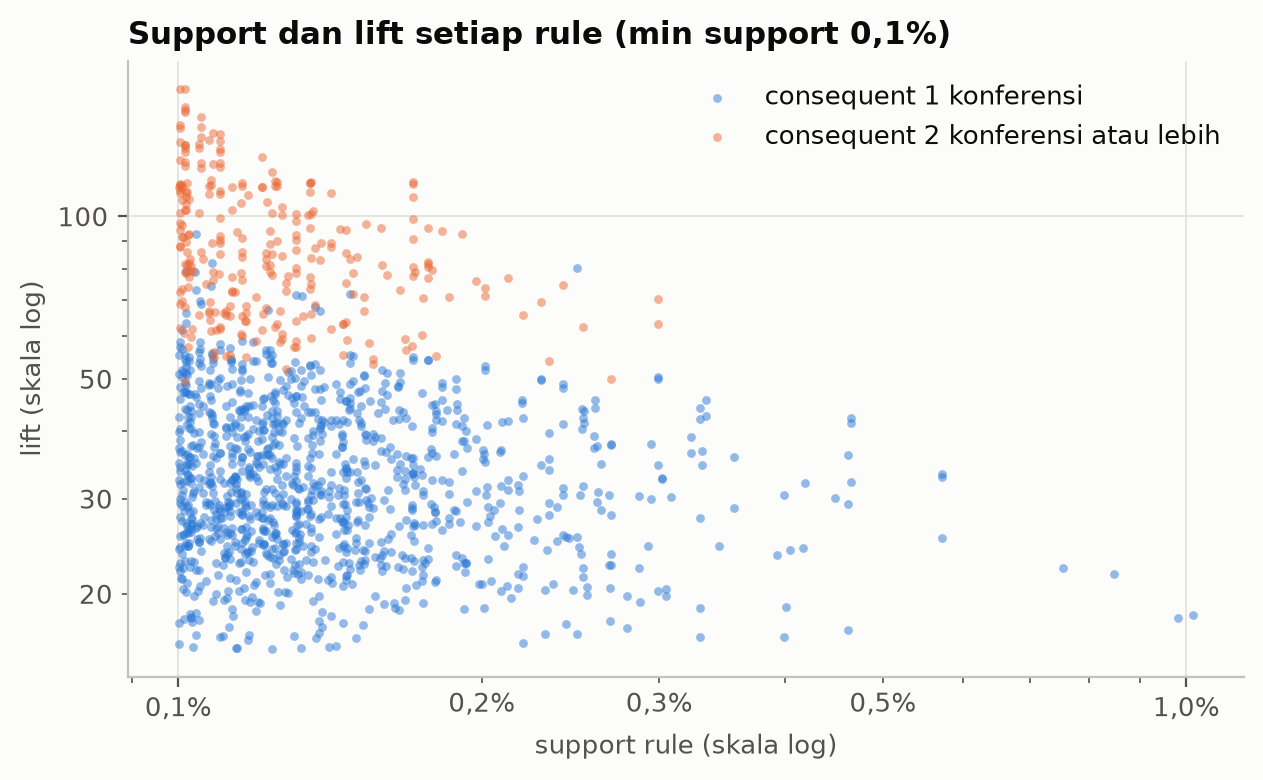
\includegraphics[width=0.9\textwidth]{images/hasil/t5_support_vs_lift.png}
\caption{\textit{Support} dan \textit{lift} setiap \textit{rule} pada \textit{min\_sup} 0,1\%}
\label{fig:t5-scatter}
\end{figure}

Pada tingkat konferensi, untuk setiap konferensi yang menjadi \textit{consequent} tunggal dihitung \textit{support}-nya dan median \textit{lift} \textit{rules} yang menuju kepadanya (Gambar~\ref{fig:t5-lift-konferensi}). Korelasi Spearman antara keduanya adalah $-0{,}933$ pada 26 konferensi. NeurIPS, konferensi dengan \textit{support} tertinggi (3,17\%), menjadi \textit{consequent} pada 240 \textit{rule}, terbanyak dari semua konferensi, tetapi median \textit{lift}-nya hanya 23,61, kedua terendah setelah ICASSP (22,85). Sebaliknya, CDC (\textit{support} 0,79\%) memiliki median \textit{lift} 92,90. Sebagai \textit{antecedent} tunggal, korelasinya $-0{,}517$ pada 17 konferensi.

\begin{figure}[ht]
\centering
\figtikz{fig-t5-lift-konferensi}
\caption{\textit{Support} konferensi dan median \textit{lift} \textit{rules} yang menuju kepadanya (26 konferensi, \textit{min\_sup} 0,1\%)}
\label{fig:t5-lift-konferensi}
\end{figure}

Penyebabnya ada pada rumus \textit{lift}, yaitu \textit{confidence} dibagi \textit{support} konferensi tujuan. Konferensi besar sudah memiliki \textit{support} tinggi sehingga \textit{rule} yang menuju kepadanya sulit mencapai \textit{lift} tinggi walaupun \textit{confidence}-nya besar. Pada data ini, \textit{lift} juga tidak berfungsi sebagai penyaring. \textit{Support} setiap konferensi di bawah 3,2\% dan \textit{min\_conf} 50\% sehingga setiap \textit{rule} otomatis memiliki \textit{lift} minimal sekitar $0{,}5/0{,}0317 \approx 15{,}8$; \textit{lift} terendah yang ditemukan adalah 15,83. \textit{Lift} dipakai untuk mengurutkan kekuatan hubungan, bukan untuk memisahkan hubungan positif dan negatif.

\subsection{Interpretasi \textit{support}, \textit{confidence}, dan \textit{lift}}
\label{sec:hasil-t5-metrik}
Tabel~\ref{tab:t5-contoh} menunjukkan tiga \textit{rule} nyata beserta \textit{count} di balik ketiga ukuran.

\begin{table}[ht]
\caption{Tiga contoh \textit{rule} dan \textit{count} di balik ukurannya}
\label{tab:t5-contoh}
\footnotesize
\begin{tabularx}{\textwidth}{@{}>{\raggedright\arraybackslash}Xrrrrrrr@{}}
\toprule
\textbf{\textit{Rule}} & \textbf{$X \cup Y$} & \textbf{$X$} & \textbf{$Y$} & \textbf{\textit{Support}} & \textbf{\textit{Conf.}} & \textbf{\textit{Support}($Y$)} & \textbf{\textit{Lift}} \\
\midrule
ICML $\Rightarrow$ NeurIPS & 18.503 & 31.896 & 57.800 & 1,016\% & 58,0\% & 3,17\% & 18,28 \\
ECOC $\Rightarrow$ OFC & 4.530 & 6.815 & 15.115 & 0,249\% & 66,5\% & 0,83\% & 80,12 \\
ECCV + ACM Multimedia + NeurIPS $\Rightarrow$ AAAI + CVPR + ICCV & 1.827 & 2.983 & 6.477 & 0,100\% & 61,2\% & 0,36\% & 172,27 \\
\bottomrule
\end{tabularx}
\end{table}

Pada \textit{rule} ICML $\Rightarrow$ NeurIPS, \textit{support} 1,016\% menyatakan seberapa umum kombinasi ICML dan NeurIPS di antara seluruh penulis. \textit{Support} tidak memiliki arah: NeurIPS $\Rightarrow$ ICML memiliki \textit{support} yang sama. \textit{Confidence} 58,0\% menyatakan bahwa dari 31.896 penulis ICML, 58\% juga menerbitkan di NeurIPS. \textit{Confidence} memiliki arah: NeurIPS $\Rightarrow$ ICML hanya 32,0\% dan tidak menjadi \textit{rule}. \textit{Lift} 18,28 menyatakan bahwa penulis ICML 18 kali lebih mungkin menerbitkan di NeurIPS dibanding penulis pada umumnya. \textit{Lift} tidak memiliki arah. Ketiga contoh memperlihatkan bahwa ketiga ukuran menjawab pertanyaan berbeda: ICML $\Rightarrow$ NeurIPS memiliki \textit{support} terbesar tetapi \textit{lift} terkecil, sedangkan \textit{rule} panjang memiliki \textit{support} terkecil (tepat di atas ambang) tetapi \textit{lift} terbesar. \textit{Support} menjawab seberapa sering, \textit{confidence} menjawab seberapa sering B jika A, dan \textit{lift} menjawab seberapa kuat hubungan A dan B dibanding jika keduanya tidak berkaitan.

\subsection{Pola publikasi antarkonferensi}
\label{sec:hasil-t5-pola}
Setiap \textit{rule} satu-ke-satu diperlakukan sebagai garis yang menghubungkan dua konferensi, lalu konferensi yang terhubung, langsung maupun lewat konferensi lain, digabung menjadi satu kelompok. Hasilnya delapan kelompok yang tidak saling terhubung (Tabel~\ref{tab:t5-kelompok}). Pembentukan kelompok berasal dari data. Nama bidang pada kolom pertama adalah pengetahuan umum penulis laporan yang dicocokkan dengan judul prosiding pada data DBLP (\texttt{venue\_proceedings.csv}), misalnya \textit{Computer Vision}, \textit{Computational Linguistics}, \textit{Machine Learning}, \textit{Communications}, \textit{Optical Communications}, \textit{Speech Recognition}, \textit{Robotics and Automation}, dan \textit{Human Factors in Computing Systems}.

\begin{table}[ht]
\caption{Kelompok konferensi dari \textit{rules} satu-ke-satu (\textit{min\_sup} 0,1\%)}
\label{tab:t5-kelompok}
\small
\begin{tabularx}{\textwidth}{@{}l>{\raggedright\arraybackslash}Xr>{\raggedright\arraybackslash}p{3.6cm}@{}}
\toprule
\textbf{Bidang} & \textbf{Konferensi} & \textbf{\textit{Rules}} & \textbf{\textit{Lift} tertinggi} \\
\midrule
\textit{Computer vision} & CVPR, ICCV, ECCV, BMVC, ACCV, 3DV & 5 & 3DV $\Rightarrow$ CVPR (25,02) \\
NLP & ACL, EMNLP, NAACL-HLT, EACL, IJCNLP-AACL & 6 & EACL $\Rightarrow$ ACL (36,59) \\
\textit{Machine learning} & NeurIPS, ICML, ICLR, AISTATS, UAI & 5 & AISTATS $\Rightarrow$ ICML (30,44) \\
Telekomunikasi & ICC, GLOBECOM, SPAWC & 2 & SPAWC $\Rightarrow$ ICC (36,23) \\
Komunikasi optik & OFC, ECOC & 1 & ECOC $\Rightarrow$ OFC (80,12) \\
Pengenalan suara & INTERSPEECH, ASRU & 1 & ASRU $\Rightarrow$ INTERSPEECH (74,17) \\
Robotika & ICRA, CoRL & 1 & CoRL $\Rightarrow$ ICRA (37,11) \\
Interaksi manusia-komputer & CHI, DIS & 1 & DIS $\Rightarrow$ CHI (33,99) \\
\bottomrule
\end{tabularx}
\end{table}

Dari 1.114 \textit{rule} dengan \textit{consequent} satu konferensi, 21,5\% menuju NeurIPS, 17,0\% menuju AAAI, dan 14,4\% menuju CVPR. AAAI tidak menjadi tujuan \textit{rule} satu-ke-satu mana pun, tetapi menjadi tujuan 189 \textit{rule} dari kombinasi dua konferensi atau lebih. Artinya, menerbitkan di satu konferensi tertentu belum cukup untuk memperkirakan seorang penulis juga menerbitkan di AAAI, tetapi penulis yang menerbitkan di beberapa konferensi \textit{machine learning} dan \textit{computer vision} sekaligus sangat mungkin juga menerbitkan di AAAI.

Sepuluh \textit{rule} dengan \textit{lift} tertinggi perlu dibaca hati-hati. Selain \textit{count}-nya hanya sedikit di atas ambang, 54 sampai 60 penulis pendukung setiap \textit{rule} itu berasal dari 291 transaksi dengan 100 konferensi atau lebih, yang hampir seluruhnya nama umum tanpa nomor disambiguasi. Tanpa transaksi tersebut, tujuh dari sepuluh \textit{rule} itu tidak lagi lolos \textit{min\_sup} 0,1\%. Hasil tetap dilaporkan apa adanya.

\subsection{Jawaban pertanyaan \textit{Task} 5}
\label{sec:jawab-t5}
\textbf{Pembangkitan \textit{rules}.} Dengan \textit{min\_conf} 50\% diperoleh 1.387 \textit{rules} pada \textit{min\_sup} 0,1\%, 7 pada 0,5\%, 1 pada 1\%, dan 0 pada 2\%, identik dengan \texttt{mlxtend}. Hanya 22 \textit{rules} pada 0,1\% yang berbentuk satu-ke-satu.

\textbf{\textit{Support}, \textit{confidence}, dan \textit{lift}.} Ketiga ukuran dihitung untuk setiap \textit{rule}. Sepuluh \textit{lift} tertinggi dipimpin ECCV + ACM Multimedia + NeurIPS $\Rightarrow$ AAAI + CVPR + ICCV (\textit{lift} 172,27, \textit{confidence} 61,2\%, \textit{support} 0,100\%).

\textbf{Hubungan paling menarik.} Tidak ada pasangan yang berlaku dua arah. \textit{Lift} tertinggi pada \textit{rule} satu-ke-satu dimiliki ECOC $\Rightarrow$ OFC (80,12) dan ASRU $\Rightarrow$ INTERSPEECH (74,17). Hubungan yang paling mendekati timbal balik adalah CVPR dengan ICCV dan ECCV, serta NeurIPS dengan ICML dan ICLR (\textit{confidence} arah balik 28,9\% sampai 32,4\%).

\textbf{\textit{Support} tinggi dan \textit{lift}.} \textit{Support} tinggi tidak menghasilkan \textit{lift} tinggi, justru sebaliknya. Korelasi Spearman antara \textit{support} konferensi dan median \textit{lift} \textit{rules} yang menuju kepadanya adalah $-0{,}933$. NeurIPS memiliki \textit{rules} terbanyak (240) tetapi median \textit{lift}-nya termasuk terendah (23,61).

\textbf{Perbedaan interpretasi.} \textit{Support} mengukur seberapa umum kombinasi di antara seluruh penulis dan tidak berarah. \textit{Confidence} mengukur peluang menerbitkan di Y di antara penulis X dan berarah. \textit{Lift} mengukur kekuatan hubungan dibanding jika X dan Y tidak berkaitan dan tidak berarah.

\textbf{Pola publikasi.} \textit{Rules} satu-ke-satu membentuk delapan kelompok bidang tanpa hubungan antarkelompok. Di dalam kelompok, arahnya selalu dari konferensi yang lebih kecil ke konferensi yang lebih besar, dan kombinasi beberapa konferensi paling sering mengarah ke NeurIPS, AAAI, dan CVPR.
